\documentclass{beamer}
\mode<presentation>
{
  \usetheme{default}
  \usecolortheme{default}
  \usefonttheme{default}
  \setbeamertemplate{navigation symbols}{} \setbeamertemplate{caption}[numbered]
} 

\usepackage{xcolor}
\usepackage[english]{babel}
\usepackage{tikz}
\usetikzlibrary{arrows,calc,through,backgrounds,matrix,decorations.pathmorphing,positioning}

\title{Inferring Bitcoin Gossip Topology}
\author{Keyhan and Alex}
\institute{CS 261}
\date{\today}

\newcommand{\advat}[1]{\node (Adv) at #1 {$\color{red}{\bullet}$} ;}
\newcommand{\nodeat}[2]{\node (#1) at #2 {$\bullet$} ;} 
\newcommand{\connect}[3][]{\draw[#1] (#2)--(#3) ;}
\newcommand{\inv}[4][above]{\draw[->] (#2)--(#4) node[midway,#1] {$\texttt{INV}$(#3)} ;}
\newcommand{\getdata}[4][above]{\draw[->] (#2)--(#4) node[midway,#1] {$\texttt{GETDATA}$(#3)} ;}
\newcommand{\tx}[4][above]{\draw[->] (#2)--(#4) node[midway,#1] {$\texttt{TX}$(#3)} ;}
\newcommand{\knows}[3][below]{\node[#1= 0.1 of #2] (#1-#2) {#3} ;}

\begin{document}

\begin{frame}
  \titlepage
  \begin{overlayarea}{0cm}{0cm}
  \begin{center}
  \vspace{-5cm}
      \includegraphics[width=2cm]{BC_Logo_.png}
  \end{center}
  \end{overlayarea}
\end{frame}

\section{Introduction}

\begin{frame}{Introduction}

\begin{itemize}
  \item Bitcoin uses a \textbf{gossip network} in order to communicate \pause
  \item In a gossip network, you broadcast your messages to your peers, \pause and then those peers broadcast your messages to their peers, \pause and then those peers broadcast your messages to their peers, \ldots \pause until you reach the whole network \pause
  \item Don't need connect to the whole network, only to our peers\pause
\end{itemize}
\begin{center}
    \includegraphics[width=5cm]{gossip.png}
\end{center}
\end{frame}

\begin{frame}{Broadcasting a Transaction}
    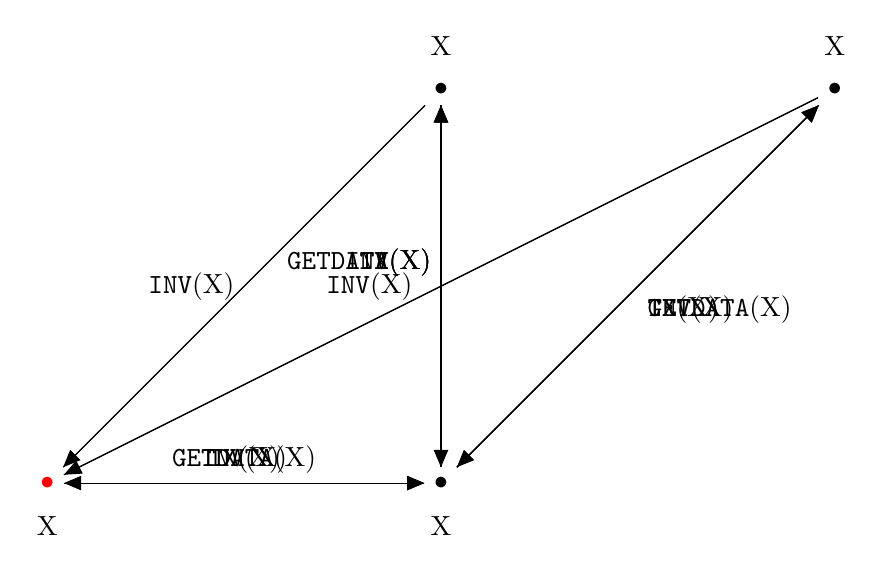
\begin{tikzpicture}[>=triangle 45]
        \advat{(0,0)}
        \nodeat{N1}{(5,5)}
        \nodeat{N2}{(5,0)}
        \nodeat{N3}{(10,5)}
        \connect{Adv}{N1}
        \connect{Adv}{N2}
        \connect{Adv}{N3}
        \connect{N1}{N2}
        \connect{N2}{N3}
        \visible<2>{\inv{Adv}{X}{N2}}
        \visible<2->{\knows{Adv}{X}}
        \visible<3>{\getdata{N2}{X}{Adv}}
        \visible<4>{\tx{Adv}{X}{N2}}
        \visible<4->{\knows{N2}{X}}
        \visible<5>{\inv[above left]{N2}{X}{N1}}
        \visible<5>{\inv[below right]{N2}{X}{N3}}
        \visible<6>{\getdata[above left]{N1}{X}{N2}}
        \visible<6>{\getdata[below right]{N3}{X}{N2}}
        \visible<7>{\tx[above left]{N2}{X}{N1}}
        \visible<7>{\tx[below right]{N2}{X}{N3}}
        \visible<7->{\knows[above]{N1}{X}}
        \visible<7->{\knows[above]{N3}{X}}
        \visible<9>{\inv[left]{N1}{X}{Adv}}
        \visible<9>{\inv[left=0.24cm]{N3}{X}{Adv}}
        \visible<10>{}
    \end{tikzpicture}
\end{frame}

\begin{frame}{Goal \& Motivation}
\begin{itemize}
    \item We want to infer the \textit{topology} of gossip networks\pause
    \begin{itemize}
        \item i.e., who is connected to whom \pause
        \item Focusing on Bitcoin servers; ignoring clients, private mining networks, etc. \pause
    \end{itemize}
    \item What might this be useful for? \pause
    \begin{itemize}
    % TODO(kvakil): Add sources for the below
        \item Deanonymization: link Bitcoin addresses with IP of server \pause
    \end{itemize}
\begin{center}\includegraphics[width=10cm]{sheep.png}\end{center}\pause
    \begin{itemize}
        \item Monopolize a target's connections, present a modified blockchain \pause
        \item Partition the network, fork the blockchain
    \end{itemize}
\end{itemize}
\end{frame}

\section{Prior Work \& Our Contributions}

\begin{frame}{Prior Work}

\begin{itemize}
\item One idea: take advantage of Bitcoin's implementation flaws\pause
\begin{itemize}
    \item Coinscope (Miller et al., 2015)\pause
    % Each nodes maintains a list of peers with a lastseen timestamp. Nodes update timestamp when they talk with the peer. Adv. can get a list of peers using GETADDR. Infer peers of each node. Now fixed -- nodes don't update timestamps
    \item IP Marker Addresses (Biryukov et al., 2014)
    % Send IP addresses to a node, wait for it to gossip those IPs to its peers, and then see who connects to the IPs
\end{itemize}\pause
\item Second idea: use fundamental side-channels in gossip network\pause
\begin{itemize}
    \item Broadcast and listen for transactions, use MLE to reconstruct network (Neudecker et al., 2016)
\end{itemize}\pause
\item Our contribution falls somewhere in the middle
\end{itemize}

\end{frame}

% \begin{frame}{Our Contribution}
% 
% \begin{itemize}
% 
% \item Novel method for determining topology of Bitcoin network
% \begin{itemize}
%     \item Global adversary who can broadcast conflicting double-spend transactions
% \end{itemize}\pause
% \item Evaluate this method via simulation
% \end{itemize}
% 
% \end{frame}

\section{Inferring Topology}

\begin{frame}{Threat Model}
\begin{itemize}
    \item Our assumption: \textbf{global} adversary connected to \textbf{all} nodes
    \visible<2->{\item Reasonable? \visible<3->{Surprisingly yes.}}\\
    \begin{tikzpicture}[>=triangle 45]
        \advat{(0,0)}
        \nodeat{N1}{(5,5)}
        \nodeat{N2}{(5,0)}
        \nodeat{N3}{(10,5)}
        \connect[color=red]{Adv}{N1}
        \connect[color=red]{Adv}{N2}
        \connect[color=red]{Adv}{N3}
        \connect{N1}{N2}
        \connect{N2}{N3}
    \end{tikzpicture}
\end{itemize}
\end{frame}

% \begin{frame}{First Idea: Returned Invites}
%     \begin{tikzpicture}[>=latex]
%         \advat{(0,0)}
%         \nodeat{N1}{(5,5)}
%         \nodeat{N2}{(5,0)}
%         \nodeat{N3}{(10,5)}
%         \connect{Adv}{N1}
%         \connect{Adv}{N2}
%         \connect{Adv}{N3}
%         \connect{N1}{N2}
%         \connect{N2}{N3}
%         \knows{Adv}{X}
%         \knows{N2}{X}
%         \knows[above]{N1}{X}
%         \knows[above]{N3}{X}
%         \inv[left]{N1}{X}{Adv}
%         \inv[left]{N3}{X}{Adv}
%     \end{tikzpicture}
% \end{frame}

\begin{frame}{Classical Idea: First Timestamp Estimator}
\begin{itemize}
    \item \textsc{Goal:} Given a node $T$, determine \textbf{direct} peers of $T$. (Simplification of general topology inference)\pause
    \item \textsc{Idea:} Send a test transaction to $T$, the first node to send an \texttt{INV} to Adversary is a direct peer\pause
    \item But Bitcoin adds Poisson noise to gossip\pause
\end{itemize}
\begin{center}
    \begin{tikzpicture}[>=triangle 45]
        \advat{(5,2.5)}
        \nodeat{W}{(0,2.5)}
        \nodeat{E}{(10,2.5)}
        \nodeat{N}{(5,5)}
        \connect{W}{N}
        \connect{E}{N}
        \connect{Adv}{W}
        \connect{Adv}{E}
        \connect{Adv}{N}
        \knows[below]{E}{Target}
        \only<5>{\tx[above]{Adv}{X}{E}}
        \only<6>{\tx[above=0.3cm]{E}{X}{N}}
        \only<7>{\tx[above=0.3cm]{N}{X}{W}}
        \only<8>{\inv[above]{W}{X}{Adv}}
        \only<9>{\inv[below right=0.03cm]{N}{X}{Adv}}
    \end{tikzpicture}
\end{center}
\begin{itemize}
\vspace{-3pt}
    \visible<10->{\item Simulated Bitcoin network ($2^9$ nodes): 31\% precision}
\end{itemize}
\end{frame}

\begin{frame}{Our Attack}
\begin{itemize}
    \item \textsc{Insight:} Bitcoin nodes \textbf{drop} attempted double spend transactions and do not share them with their neighbors\pause\end{itemize}
\begin{center}
    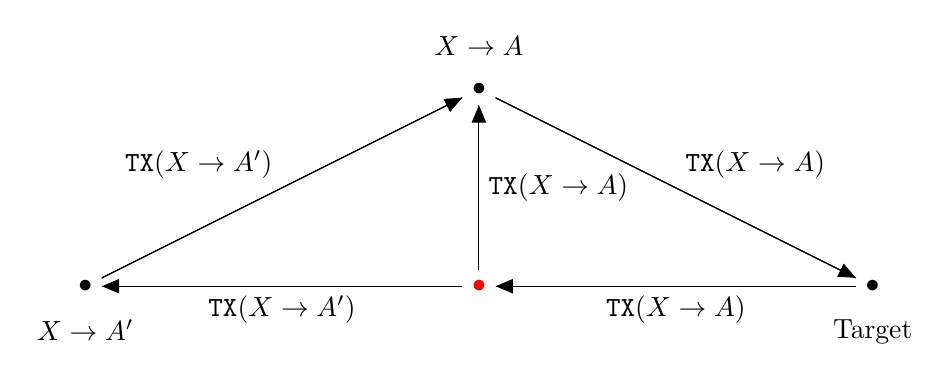
\begin{tikzpicture}[>=triangle 45]
        \advat{(5,2.5)}
        \nodeat{W}{(0,2.5)}
        \nodeat{E}{(10,2.5)}
        \nodeat{N}{(5,5)}
        \connect{W}{N}
        \connect{E}{N}
        \connect{Adv}{W}
        \connect{Adv}{E}
        \connect{Adv}{N}
        \knows[below]{E}{Target}
        \visible<3>{\tx[right]{Adv}{$X \to A$}{N}}
        \visible<3>{\tx[below]{Adv}{$X \to A'$}{W}}
        \visible<4->{\knows[below]{W}{$X \to A'$}}
        \visible<4->{\knows[above]{N}{$X \to A$}}
        \visible<5>{\tx[above left]{W}{$X\to A'$}{N}}
        \visible<7>{\tx[above right]{N}{$X \to A$}{E}}
        \visible<8>{\tx[below]{E}{$X \to A$}{Adv}}
    \end{tikzpicture}
\end{center}
\begin{itemize}
    \visible<9->{\item Broadcast conflicting transactions to entire graph (except target) $\implies$ infer a connected peer 100\% of the time}
\end{itemize}
\end{frame}

\begin{frame}{Problems}
\begin{itemize}
    \item Requires simultaneous broadcast\pause
    \item Sensitive to network latency\pause
\end{itemize}
\begin{center}\includegraphics[width=5cm]{over9000.png}\end{center}\pause
\begin{itemize}
    \item Simulation: Robust to limited delays in simultaneous broadcast and network latency\pause
    \begin{itemize}
    \item Intentional noise typically dominates other noise
    \end{itemize}
\end{itemize}
\end{frame}

\begin{frame}{Improving Efficiency}
\begin{itemize}
    \item Might infer the same connection multiple times\pause
    \begin{itemize}
        \item \textbf{Forcing Variant}: ``ignore'' a certain edge we already know, but increases TX fee cost
    \end{itemize}\pause
    \item Only infers one connection at a time\pause
    \begin{itemize}
        \item \textbf{Batching Variant}: multiple edge inference, constant bandwidth per edge, but decreases precision
    \end{itemize}
\end{itemize}
\end{frame}

\section{(Brief) Comparison to Prior Work}
\begin{frame}{Comparison to Prior Work}
\begin{itemize}
    \item $F_1$: measure of how good a detector is \pause
    \item Prior Work (Neudecker et al., 2016): $F_1 \approx 40\%$ \pause
    \item This Work: $F_1 = 1$ (if you're willing to pay for it!) \pause
    \begin{itemize}
        \item Simulation: $F_1 \approx 64\%$ after only $\approx 20$ rounds
    \end{itemize}\pause
    \item Why is this not a fair comparison?\pause
    \begin{itemize}
        \item Prior work might work with a passive attacker, our method requires an active attacker \pause
        \item Our attack is more costly, but also more effective
    \end{itemize}
\end{itemize}
\end{frame}

\section{Proposed Solutions}
\begin{frame}{Proposed Solutions}
\begin{itemize}
    \item New Gossip Network: Dandelion(++)\pause
\end{itemize}
\begin{center}\includegraphics[width=5cm]{Dandelion.jpg}\end{center}\pause
\begin{itemize}
    \item Broadcast conflicting transactions (always, or maybe with some probability)\pause
    \item We plan to analyze some of these for our final report
\end{itemize}
\end{frame}


\section{Q\&{}A}
\begin{frame}{Thanks!}
    \begin{itemize}
        \item Code on Github: \url{https://github.com/kvakil/261-project}
        \item Questions? Feedback?
    \end{itemize}
\end{frame}

\section{Extra Slides (if time)}

\begin{frame}{Forcing}
\begin{itemize}
    \item \textsc{Goal:} Given a node $T$ and an already-known peer $S$, determine direct peers of $T$ \textbf{excluding $S$}
    \item Say that we have two bitcoins\footnote{Now we really mean UTXOs.} $X$ and $Y$.
    \begin{enumerate}
        \item For each $n_i \neq S, T$, create a transaction $t_i$ which sends bitcoin $X$ to a different address.
        \item For $S$, create a transaction $t_S$ which sends bitcoins $X$ \& $Y$ to an address $A$. 
        \item For $T$, create a transaction $t_T$ which sends bitcoin $Y$ to an address $A' \neq A$.
        \item Simultaneously broadcast transaction to each node
        \item Eventually, $T$ will send back $\texttt{INV}(t_i)$ to the adversary. Deduce that $T$ is directly connected to $n_i\neq S$.
    \end{enumerate}
    \item $T$ cannot accept $t_S$, since $t_S$ conflicts with $t_T$.
\end{itemize}
\end{frame}

\begin{frame}{Batching ($\texttt{recv} > 1$)}
\begin{itemize}
\item \textsc{Goal:} Generalize previous attack to infer multiple connections at once
\item \textsc{Insight:} Have multiple nodes which don't receive transactions
\item Partition network nodes into two sets, $\texttt{recv}$ and $\texttt{send}$. Say that we have 1 bitcoin.
\begin{enumerate}
    \item For each $n_i \in \texttt{send}$, create a transaction $t_i$ which spends the bitcoin. Each $t_i$ sends the bitcoin to a different address.
    \item Simultaneously broadcast $t_i$ to each node in $\texttt{send}$.
    \item Eventually each node $T \in \texttt{recv}$ will send back $\texttt{INV}(t_i)$ for some $i$. Deduce that $T$ is directly connected to $n_i$.
\end{enumerate}
\item Tradeoff: no longer 100\% sure of connections
\end{itemize}
\end{frame}

\end{document}
